\section{Switching Waveforms and ZVS}
\label{sec:res-zvs}

The MCU burst-enable pin PA10 groups the nominal \SI{1}{\mega\hertz}
carrier into packets. Figure~\ref{fig:pdo20-high-power-scope} shows the
switch-node and output voltages in the high-power tests. The raw C2
waveforms show burst structure and individual switching transitions.

\begin{figure}[htbp]
\centering
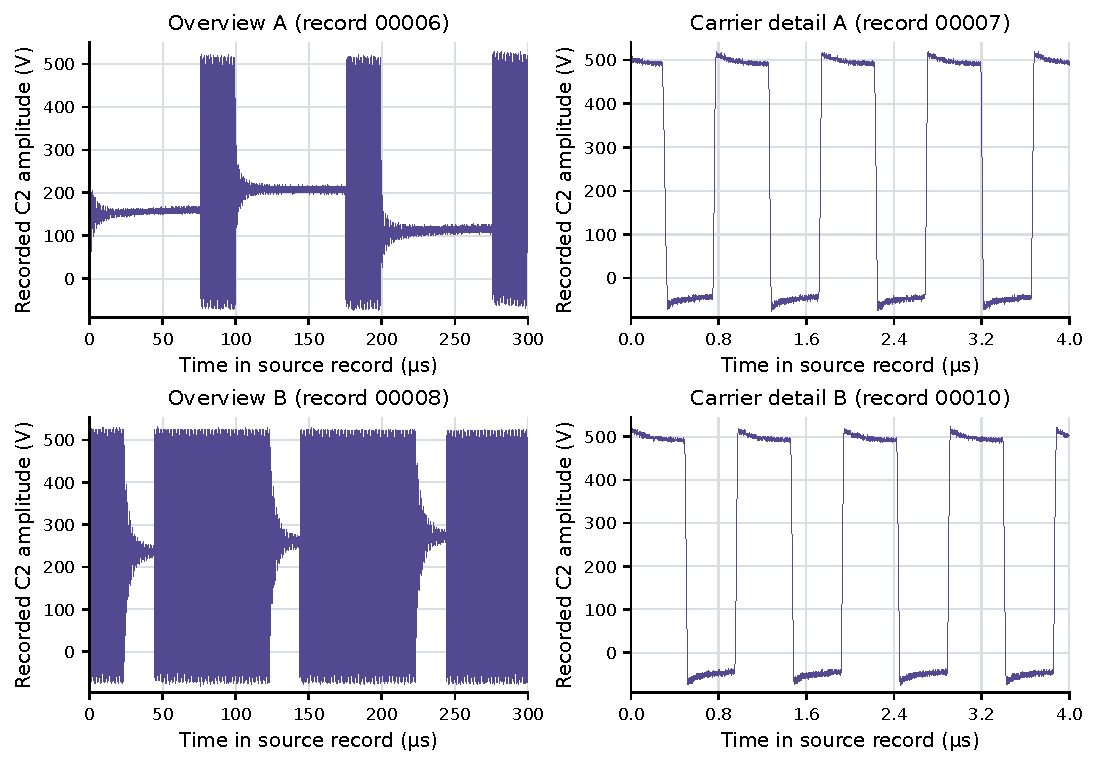
\includegraphics[width=\textwidth]{Pictures/Thesis/10_Results/Rebuilt/raw_switching_records.pdf}
\caption{C2 waveforms showing burst overviews (00006 and 00008) and carrier detail (00007 and 00010).}
\label{fig:switching-waveform-evidence}
\label{fig:rebuilt-raw-switching}
\end{figure}
\FloatBarrier

The overview records show packets followed by ringing toward an intermediate
node voltage. Switching occupies more of the displayed interval in record 00008 than
in record 00006. In the detail views, the median spacing between rising transitions detected
with hysteresis is about \SI{0.967}{\micro\second}, corresponding to
approximately \SI{1.03}{\mega\hertz}. This is the frequency measured in the C2
waveforms; the configured timer frequency and test conditions were not recorded.

The resonant current can discharge half-bridge capacitances before turn-on
\cite{ammar2020chargepump,ammar2021led}. Turn-on voltage is measured
from the incoming device's gate-source transition and drain-source voltage
on the same calibrated time base. The quantity
\begin{equation}
V_\mathrm{DS,res}=V_\mathrm{DS}(t_\mathrm{gate,on})
\end{equation}
has to be evaluated when the gate reaches a stated turn-on threshold.
The single-node captures do not locate that instant.

\begin{table}[htbp]
\centering
\caption{Switching-waveform observations and missing measurements.}
\label{tab:zvs-results}
\begin{tabularx}{\textwidth}{@{}L{0.31\textwidth}X@{}}
\toprule
Capture & Observation or missing measurement\\
\midrule
Main DC-coupled captures & Switching and output-bus behavior at identified loads\\
Raw overview and detail records & Burst structure and approximately \SI{1.03}{\mega\hertz} carrier activity in the exported records\\
Gate-source timing and deskew missing & Residual turn-on voltage and actual dead time cannot be measured from these captures\\
\bottomrule
\end{tabularx}
\end{table}

ZVS remains unverified, particularly at packet boundaries. Classification
requires gate-referenced turn-on captures with known probe loading, return
inductance, deskew, and amplitude calibration.
